\documentclass[journal]{IEEEtran}

\ifCLASSINFOpdf
\usepackage[dvips]{graphicx}
\DeclareGraphicsExtensions{.pdf,.jpeg,.png}
\else
\fi

\usepackage[cmex10]{amsmath}
\interdisplaylinepenalty=2500
\usepackage{algorithmic}
\usepackage{array}

\ifCLASSOPTIONcompsoc
\usepackage[caption=false,font=normalsize,labelfont=sf,textfont=sf]{subfig}
\else
\usepackage[caption=false,font=footnotesize]{subfig}
\fi

\usepackage{fixltx2e}
\usepackage{url}
\usepackage{amsfonts}
\usepackage{graphicx}
\usepackage{multirow}
\DeclareMathOperator*{\argmin}{argmin}
\usepackage[colorlinks=true,
			citecolor=blue,
			linkcolor=blue,
			urlcolor==blue]
			{hyperref}

\usepackage{soul}

\begin{document}

\title{Bayesian estimation of the residential baseline}

\author{Pierre-Andre~Cornillon,
Andrew~Frazer,
Nicolas~Hengartner, 
and Eric~Matzner-L{\o}ber
\thanks{P-A. Cornillon is with , e-mail: }%
\thanks{A. Frazer is with Los Alamos National Laboratory, USA, e-mail: }%
\thanks{Nick Hengartner is with Los Alamos National Laboratory, USA, e-mail: nick@lanl.gov}%
\thanks{E. Matzner-L{\o}ber is with CREST, ENSAE-CEPE, France, e-mail: eml@ensae.fr.}
}
\maketitle

\begin{abstract}

\end{abstract}

\begin{IEEEkeywords}
Demand reduction, Energy management, Load management, Control group, Baseline estimation
\end{IEEEkeywords}

\IEEEpeerreviewmaketitle

\section{Introduction}\label{sec:intro}
{\bf NEEDS TO MODIFY and tell a story according to Los Alamos....}
\IEEEPARstart{L}{iberalization} of the electricity markets mainly led
to the reorganization of the electricity companies. While vertically
integrated markets are supply-side mechanisms, open markets are
demand-side systems \cite{IEA}. So, instead of responding to all
demand variations and supporting the price volatility, the new
philosophy consists in reducing the demand fluctuations by subjecting
the customers to price variations \cite{def_DR}.  This especially
leads to incite customers to lower their peak consumption. This
mechanism is demand response (DR). DR appeals to customers to reduce,
shift or shed their peak consumption by modifying their behavior. To
this end, \emph{tariff incentives} are classical solutions. One
alternative is to manage flexible electrical appliances by
\emph{direct load control}. Thus, DR results in new flexible solutions
allowing to:
\begin{itemize}
\item maintain the reliability of the electric system efficiently and at a lower cost,
\item lower the wholesale market prices by managing the electricity demand through demand reduction.
\end{itemize}  

\noindent Moreover, since the grid reliability is improved by peak demand reductions,
the reduced use of polluting peaking plants (coal turbines) may provide environmental benefits.

To integrate DR in the whole electricity system, many countries around the world 
investigated DR programs on industrial, commercial and residential customers. In 
this paper, we mainly focus on the residential sector. DR experiments 
tested tariff incentives with dynamic pricing \cite{REX_DP} and direct load control 
of the electrical appliances, such as air-conditioners (AC) or heaters \cite{DECC_literature}.
Combined demonstration studies proved that these flexible usages 
can provide a significant source of demand reduction \cite{Rex_baseline} (Fig. \ref{effacement}).
\begin{figure}[!h]
\centering
\includegraphics[width=3.5in,height=2in]{baseline} 
\caption{{\scriptsize Characterization of a residential demand reduction between 6 and 8 pm on 
a small customers group.}}
\label{effacement}
\end{figure}

The total residential demand reductions can be currently enhanced on electricity 
markets and incorporated in the grid operations. As new entrants on the energy markets, load 
aggregators or curtailment service providers are developing DR offers. Hence, a customer's 
load reduction becomes a paid resource. To this end, the demand reduction has to be 
evaluated. This is a difficult problem
since it is impossible to measure it, the only available measure is the consumption obtained
with the DR program. So to quantify the curtailment, one has to estimate the 
consumption, called the baseline, which would have been used in the absence of this demand 
reduction. The curtailment is then obtained by subtracting the metered load during the 
demand reduction event from the baseline (Fig. \ref{baseline}). 
\begin{figure}[!h]
\centering
\includegraphics[width=3.5in,height=2in]{baseline} 
\caption{{\scriptsize Los ALAMOS DATA}}
\label{baseline}
\end{figure}
Developing accurate baseline estimation methods, remunerating customers and 
including DR resources in planning operators is becoming a major issue for all electricity 
stakeholders.  

Many baseline methods stem from experiments carried out. Among the first ones developed 
for Independent System Operators (ISO) in non-residential building \cite{eval_baseline}, day or
weather matching methods are the most common. More recently, regression models were tested on
commercial and industrial buildings \cite{quantifying_berk}. 
In econometric research, it is largely advocate to use randomized controlled field trials
to evaluate the residential average treatment impact \cite{energy_efficiency_gap}.
While many DR pilots use randomized experiments to estimate residential demand reduction
or programs impacts, others encounter some constraints and specify a non-experimental
estimate (i.e. control group). 

As mentioned in many papers \cite{behavorial_energy_policy,social_norms} and studies
\cite{Rex_baseline,experimental_evidence}, 
having a control group can be important to estimate the baseline. Unlike matching 
or regression methods, control group based methods are well adapted to evaluate the residential load
curve and estimates provide more accurate results \cite{Rex_baseline}. Nevertheless, deploying 
a control group for a commercial use is not appropriate because all recruited customers 
are enrolled in the DR offer and reduce their demand.  


Electric utilities often have representative residential portfolio
database with individual load curves and characteristics. Besides, to
enable the DR on the markets, many technological improvements were
done and advanced metering infrastructure were developed, such as
smart meters. Therefore, a certain amount of individual load curves
are recorded every day and are available to be used. Electricity load
curves largely reflect the customers behavior and individual load
curves are characteristic of the rate type, the heating or AC use, the
daily consumption, and so on. In this paper, we present a new control
group selection method based on individual load curves. The solution
aims at selecting individuals from the data-mart such that the
distance between the selected control group load curve and that of the
DR group is minimal. Our approach is different then the one proposed
by \cite{directestimation}. We focus on a Bayesian strategy. Our methodology does not require
a long history to estimate the baseline and allow to estimate the baseline and could give
confidence intervals associated to the estimation. To our knowledge, this is new.

Section \ref{sec:current} reviews the current control group selection
methods and discusses their limits. In section \ref{sec:new} we expose
in details our new methods and apply it to Los Alamos data.


\section{Current control group selection methods}\label{sec:current}
\subsection{Randomized control groups}
Randomized experiments are common practices to evaluate the effects of a 
treatment in clinical trials, employment and training programs, 
labor market policies, and so on \cite{behavorial_energy_policy}. Randomized  
experiments aim at confirming on a small scale and 
under control one or many hypothesis. This approach was used in the first 
DR experiments \cite{Rex_expe_mondiales}, mainly to
evaluate feedback programs' impacts.

The objective of a randomized experiment is to build two identical groups in the way 
that one controls the other. Having a control group allows to control 
all of the parameters in order to verify that the observed 
effects, i.e. the demand reductions, arise only from the applied treatment, i.e. 
the DR lever. Then, prior to the experiment, it is fundamental that the DR group 
(the treatment group) and the control group be similar on all dimensions: the variable 
of interest, i.e. their load curve, and their individual characteristics. This sets 
important conditions on the control group customers recruitment which constitutes a 
major issue to statistically validate the impacts of the tested DR levers. 
To ensure that the trial results do not depend on the selected control customers, one of the most 
important conditions is to recruit control and DR customers at the 
same time and within the same protocol. Generally, the recruitment relies on criteria defined 
from customers' observable individual characteristics. Accepting to participate in an 
experiment depends on the interests and advantages that the customers may have. These 
criteria are personal and in-observable, we talk about propensity. From 
the customer set having accepted to join the experiment, control and DR groups are 
built. It guarantees that the only difference between the two groups only 
stems from the treatment and not from the difference between the two 
groups \cite{behavorial_energy_policy}. Customers are allocated in each group via 
a stratified random draw according to 
their individual characteristics (accommodation, localization, electricity rate, etc.). 
Thus, the groups are both distributed evenly on the observable and in-observable 
characteristics. This limits the selection bias.

Many energy savings programs have used randomized experiments. The most popular 
are Statewide Pricing Pilot \cite{CG_california}, Anaheim Critical-Peak Pricing 
Experiment \cite{ACPPE}, Olympic Pennynsula Project \cite{OPP}, Smart Metering 
Project \cite{CERai}, the Integral Energy trial \cite{NERA}, PowerCentsDC 
Program \cite{PCDC}, Kyushu Electricity Pricing Experiment \cite{japon} and 
Energy Demand Research Project \cite{EDRP}. However, for certain electric utilities, 
randomized experiments can be a costly solution because all control customers have to be 
metered. In this case, a control group selected from non-experimental data 
is used \cite{social_norms,newsham_birt_rowlands}. In addition, to enhance 
demand reduction on the electric markets, baseline estimation methods have 
to be compatible with the operational constraints. While baseline estimation 
methods relying on randomized control groups provide accurate results 
\cite{Rex_baseline,social_norms}, deploying a randomized control group 
for an operational use is not possible. Indeed, all recruited customers would be enrolled 
in the DR offer and everyone would receive demand reductions signal. Thus, to move on to 
the large-scale and estimate the baseline on a wide DR group, a control group based on 
non-experimental data could be the solution.

\subsection{Non-experimental control groups}
Most electric utilities generally hold a data-mart containing sample groups of their 
customers portfolio. They have available individual load curves and characteristics. 
These characteristics can be the annual or daily consumption, the accommodation type (apartment or house) 
and its square footage, the electricity rate, the localization, the electrical devices, and so on. 
In general, in order to consider the propensity of the DR customers enrolled in the DR program and to 
construct an accurate control group, utilities select non-DR customers sharing as far as 
possible the same observable characteristics. If a difference persists between the DR group 
load curve and that of the selected control group, a method, detailed in section 
\ref{ssec:base_cg} and employed in the Ontario Peaksaver Program \cite{newsham_birt_rowlands}, 
consists in correcting this difference with an adjustment calculated from data of the DR and 
control group load curve. 

Although this kind of method is simple and seems not to be costly, it presents some major drawbacks. First, 
in order to select an accurate non-experimental control group, we require many individual 
characteristics which are not classically stored in the database. Collecting these data on the two 
groups of customers is costly. Secondly, individual characteristics stored in a 
database only bring a static view of the customer energy use. They are not able to take 
on board every behavioral or energy use change in the selection control group. Finally, 
most of the non-experimental methods attempt to reduce the difference between the DR and 
control group 
load curves only from the observable characteristics while a part of this difference 
stems from in-observable characteristics, expressing the customer propensity to join 
a DR offer. 

To consider both in-observable information and the energy use changes automatically, one 
solution is to base the control group selection on the individual load curves rather than 
on the individual characteristics.

\subsection{Enhancement of the control group selection}
The individual load curves implicitly provide information related to in-observable 
variables. Besides providing a lot of information, they are automatically and daily updated, 
procuring then a dynamical view of the customer energy use. Therefore, to directly take into 
account all behavioral or energy use changes, the control group selection should rely on 
the individual load curves. Thus, we developed new control group selection methods based on 
the individual load curves and allowing to include observable and in-observable information 
in the control group building.  

The aim is to select control individuals such that the distance between 
the control group load curve and that of the DR group is minimal. We suggest two methods 
presented in the next section.  

\section{Sequential selection}\label{sec:new}
In \cite{directestimation}, the authors proposed a sequential selection.
The individual load curve is a
time series denoted $P_j(t)$. In order to test ou method, we will consider that $N$
individuals are affiliated to a demand reduction program. The average load curve of
that group is given by: 
\begin{equation}\label{eq:DRcurve}
P^{DR}(t)=\frac{1}{N}\sum_{j=1}^N P_j^{DR}(t)
\end{equation}
where $P_j^{DR}(t)$ is the load curve of the individual $j$ belonging to the DR program 
(example on Fig. \ref{DR_gp}).
\begin{figure}[!h]
\centering
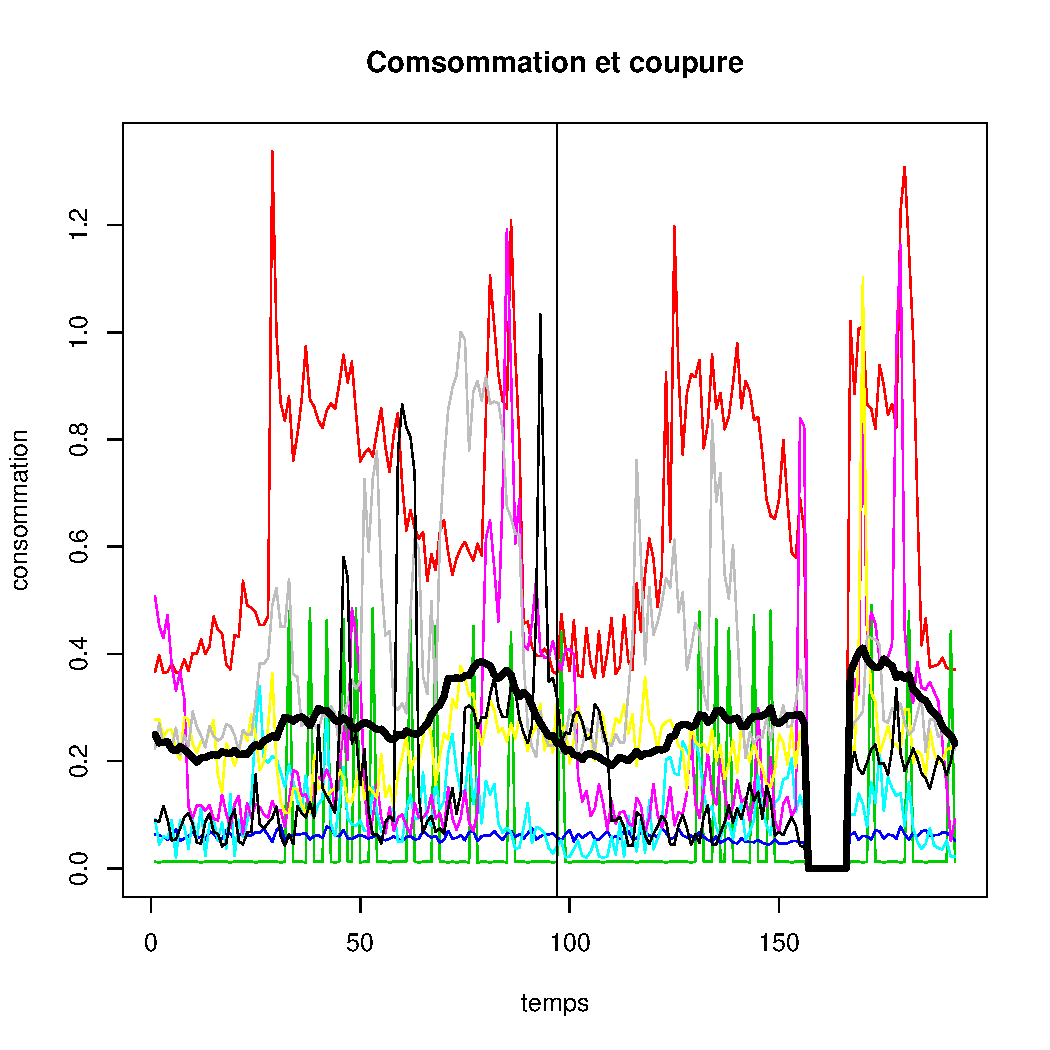
\includegraphics[width=3.5in,height=2in]{DR_gp}
\caption{{\scriptsize The different dotted and dashed lines exhibiting different
variabilities characterize the individual 2-days DR load curves. Their average load
curve is the bold solid line, representing the DR group load curve. Demand reductions
are called between 6 and 8 pm on the days 11 and 12.}}
\label{DR_gpe2}
\end{figure}
Electric utilities hold data-mart containing $M$ non-DR customers and their individual 
load curves denoted $V_i(d,t)$ or for simplifation reason $V_i$. Our aim is to construct
a control group load curve $P^{C}(d)$ to estimate the baseline on event days (example
on Fig. \ref{CG_gpe2}). 
\begin{figure}[!h]
\centering
\includegraphics[]{CG_gpe2}
\caption{{\scriptsize Representation of the 3-days individual load curves (dotted
and dashed lines) usable as control load curves. The average load curve of the selected
control group is the bold solid line.}}
\label{CG_gpe2}
\end{figure}
The objective consists in selecting some of those individuals such that
\begin{equation}\label{generalpb}
\left\|P^{DR}(\underline{t}) - P^C(\underline{t})\right\|_2
\end{equation}
be minimal, where the time sequence should be define on non event days. If we consider
as historic the day prior to the event day, the time sequence will be 96 (24 times 4)
but ones could define the time sequence. In \cite{directestimation} selected a control
group using a sequential algorithm. Once a curve is selected in the control group it has
to be remove. Their  algorithm is:
\begin{itemize}\label{eq:algo}
\item Initialization: \\
Choose the historic $t$ and evaluate: 
$$S_{1,i}=\left\|P^{DR}(t) - P_i(t)\right\|_2, ~~i_1=\argmin_{i=1,\cdots,M} \left\{S_{1,i} \right\}$$
$$P_{(1)}(t)=P_{i_1}(t),~~\hat{S_1}=\left\|P^{DR}(t)-P_{(1)}(t)\right\|_2$$ 
\item Loop on $k=2, \cdots, M$:
$$i_k= \argmin_{i \in \{1,\cdots,M\}\backslash \{i_1,\cdots,i_{k-1}\}} \left\{S_{k,i} \right\}$$
where $S_{k,i}=\left\|P^{DR}(t) - \frac{1}{k}\left[\sum_{l=1}^{k-1} P_{(l)}(t)+P_i(t)\right]\right\|_2$
$$\hat{S_k}=\left\|P^{DR}(t)-\frac{1}{k}\left[\sum_{l=1}^{k} P_{(l)}(t)\right]\right\|_2$$
\item The customers sets $\{i_1\} \subset \cdots \subset \{i_1, \cdots, i_m\} \subset \cdots \subset \{i_1, \cdots, i_m, \cdots, i_M\}$ and the respective distances $\hat{S}_1, \cdots, \hat{S}_m, \cdots, \hat{S}_M$. Select the customers set $\{i_1, \cdots, i_m\}$ minimizing the distance $\hat{S}_m$.
\end{itemize}
The selected customers set constitutes the control group of size $m$ and 
its load curve is obtained by 
$P^C(t)= \frac{1}{m} \sum_{i \in \{i_1,\cdots,i_m\}} P_i(t)$. This 
algorithm attributes a weight of $1$ if the individual $i$ is selected, $0$ if not; it is 
easily implemented with the free statistical \texttt{R} software \cite{logiciel_R}. We 
can apply this algorithm in an ascending or descending way. With modifications, identical 
load curves can be selected several times. Note that it is also possible to 
minimize the L$^1$ distance, which is more appropriate for curves. Their results were
very comparable to other methods.\\
\\

We propose in this paper a Bayesian algorithm to estimate the control group.
\section{Bayesian estimation of the control group}
So we have the aggregated load curve of the demand response group
denoted $P^{DR}(t)$, for ease of notation, let us denote $Y(t)$, and
we have $M$ individual load curve $P_i(t)$. Let $A_1,\ldots,A_m$ be $m$
indicator variables where $A_i=1$ if the $i$th curve is in the control
group. Again, this group is chosen in such a way that is mean aggregated
curve is as closed as possible to $Y(t)$. Our aim is to calculate the
conditional distribution of $A_1,\ldots,A_m$ knowing $Y(t)$. For doing
so, we are going to use a MCMC procedure. In the sequel, we will give
all the details.\\
Initialy, we suppose that the indicator variables are i.i.d Bernouilli
with parameter $p$. Given the $A_1,\ldots,A_m$ we suppose that the
demand response curve $Y(t)$ is a Gaussian process with mean
\begin{equation}
\mu(A_1,\ldots,A_m) = \sum_{j=1}^m A_j P_j(t)
\end{equation}
and variance $\sigma^2$.
The a priori distribution on $p$ is a Beta with parameters $B(\alpha_p,\beta_p)$
and the a priori distribution on $\tau = 1/\sigma^2$ is a Gamma with
parameters $\Gamma(r,\alpha)$.\\
Given the data, we can readily compute a posterior distribution for 
$A_1,\ldots,A_m$.  Denote by $A^{-k}$ the collection of all the $A$'s
without $A_k$.  Then
\begin{equation}
  {\mathbb P}[A_j = 1 | A^{-j},\tau,Y(t),p] =
  \frac{1}{1+(1-p)/p}\frac{w_j(1)}{w_j(0)+w_j(1)}, \label{curve}
\end{equation}
where 
\begin{equation}
w_j(z) = \exp(-\tau \|Y(t) - \sum_{k \not = j} A_k P_k(t) + z P_j(t)\|^2 ).
\end{equation}
Furthermore, the distribution of 
\begin{equation}
(\tau | A_1,\ldots,A_m, Y(t), p)  \sim \Gamma(r+T/2,\alpha + \|Y(t) - \sum_{k=1}^m A_k P_k(t)\|^2).
\end{equation}
where $T$ is the number of measures of the time series.
Hence we readily can sample from the posterior distribution using a Gibbs sampler.

\medskip


{\bf Initialization}\\
Let us choose $\alpha_p=\beta_p=2$ and $r=5$ and $\alpha=200$.\\
For beginning with, we simulate $m$ Bernouilli with parameter $p$ which
is approximately the proportion of individuals in the DR program compare
the the available data set. We evaluate the mean curve and compare to
$Y(t)$. From the estimation of the errors, we could initialize $\tau$.\\
Taken at random a curve $P_i(t)$, we evaluate the quantity given by
equation \ref{curve} and draw a uniform. If the latter is smaller than
the quantity evaluated teh corresponding $A_i$ equals 0, 1 otherwise.
We do that for the $M$ curves.\\
At the end of the iteration, we have $M$ new values for the $A_i$,
we estimate the average curve $\hat Y_1(t)$, the number of curves used
denoted $k_1$ and evaluate the residual sum of square (RSS) between
$\hat Y_1(t)$ and $Y(t)$. \\
{\bf Iteration}\\
We simulate a new value for $p$ by modifying the parameter of the Beta.
$\alpha_p= 2 + k_1$ and $\beta_p=2 +(m-k_1)$. For $\tau$
we use $r=5+T/2$ et $\alpha=200+RSS$. And redo the previous iteration.\\
We do that until convergence. At the end of the procedure, we have
values for $A_1,\cdots,A_M$ and propose $\hat Y(t)$. Since these
curves involved in the average are not included in the DR, they are not
impact by the DR and they coul be used for estimating the mean curve during
the DR event.

It is also possible to obtain confidence intervals



\section{OLD Results}\label{sec:res}
Since 2010, Electricit{\'e} De France (EDF) has been experimenting with the 
DR program on residential customers in Brittany. 
The ``Une Bretagne d'avance'' trial recruited volunteers to test direct 
load control on electric heating and hot water production. During the 2011-2012 winter, demand 
reductions were called on the 20 coldest days between 6 and 8 pm. To evaluate the baseline estimation methods, 
we consider these experimental data where the energy use is metered every 10 minutes. The 
studied DR group is made up by $N=280$ customers. To select the control group, we 
have $M=433$ individuals in the data-mart living in the same geographical area and having the peak 
and off-peak hours rate of the DR group. We have five control group selection methods tested on various historic periods 
$\underline{d}$. We present here results obtained with $\underline{d}=7$ 
non-event days prior to the event day $d$. We 
compare these new methods with the day and weather matching methods, the regression model 
considered in \cite{quantifying_berk} and the control group obtained from the average of the 
$M$ individual control loads described previously. As we evaluate the 
methods on real data with the demand reduction event between 6 and 8 pm, we calculate 
the daily MAPE($d$) criteria, MAPE($d$)=$\frac{1}{T}\sum_{t=1}^T |\frac{\hat{y}_t-y_t}{y_t}|\times 100$, 
between 6 am and 6 pm and we estimate the standard deviation of the MAPE($d$), denoted 
$\hat{\sigma}_d$. We do not include the hours before 6 am and after 8 pm because 
demand reductions will not be called during these off-peak times and we want that 
the baseline matches at its best during probable demand reduction periods of the 
day. Moreover, considering this period 
is a useful tool to evaluate the baseline accuracy on the daily load curve 
as, in future, demand reductions could occur several times within a day. 

The results presented in Table \ref{tab:res} strengthen our idea 
of considering the individual load curves 
to select the control group. 
\renewcommand{\arraystretch}{1.3}
\begin{table}[!h]
\caption{{\scriptsize Average MAPE($d$) (and standard deviation $\hat{\sigma}_d$) evaluated 
between 6 am and 6 pm for all methods applied on the 20 event days. *Estimated on 13 
event days, none equivalent days found for the others.}}
\label{tab:res}
\centering
\begin{scriptsize}
\begin{tabular}{l|c|c|c|l|c|c}
\hline
 & \multicolumn{3}{c|}{Control group} & \multicolumn{2}{c|}{Day and weather} & \multirow{2}{*}{Regression}  \\
 \cline{2-4}
 & only & + adj. & + reg. & \multicolumn{2}{c|}{ matching} & \\
\hline
Algo L$^1$    		  & 7.23   &    7.50   &  7.27  & NE ISO    & 18.22  & 10.92 \\
					  & (2.83) &   (3.12)  & (3.84)	&			& (15.11)& (5.39)\\		
Algo L$^2$    		  & 6.99   &    7.35   &  7.26  & NY ISO    & 10.18  &       \\
					  & (2.90) &   (3.08)  & (4.00) &			& (5.20) & 		 \\	
Ridge  				  & 6.60   &    6.64   &  7.90  & CA ISO    & 10.40  &       \\
					  & (3.25) &   (3.25)  & (3.64)	&       	& (4.91) & 		 \\	
Lasso     			  & 6.18   &    6.23   &  7.49  & RTO PJM   & 8.54   &       \\
					  & (3.18) &   (3.18)  & (4.19)	&			& (3.82) & 		 \\	
\multirow{2}{1cm}{Positive Lasso}  		   & 6.75   &    6.85   &  7.37  & Weather   & 11.56* &       \\ 
				  	  & (3.53) &   (3.48)  & (4.05) &			& (5.72) & 		 \\	  
Average			  	  & 15.38  & 13.11     & 8.32   &  5 coldest days   & 7.95   &       \\
         			  & (7.89) &   (6.47)  & (4.60) &           & (2.63) &       \\
\hline
\end{tabular}
\end{scriptsize}
\end{table}
Whereas the best accuracy is obtained with the Lasso selection 
method, the algorithm results are less variable. Note that, with the new methods, 
the baseline accuracy is largely improved and the selected control group is less variable 
compared to the results obtained with the load curves average. Control group 
selection based only on observable individual characteristics is not sufficient to 
estimate the baseline accurately, there is still a systematic difference. So, 
this shows that even if individuals share the same 
characteristics, their behaviors are different. Applying an adjustment or a regression 
model to the new methods does not significantly improve the baseline accuracy. This could 
mean that a great part of the selection bias is caught by the new control group selection methods 
and, to improve the accuracy more, we may need a greater and more diversified sample 
of individual load curves usable as control loads. Finally, to estimate the baseline 
of one event day on these data, it 
is more accurate and faster to use the algorithm than the Lasso regression. Indeed, the CPU time 
consumed by a 2.4 GHz PC-Intel(R) Core(TM) i5 and the Windows 7 Professional 64 bits Operating 
System is 0.01 second (sec) for the algorithm with the L$^2$ distance (0.08 sec with the L$^1$ 
distance), 0.02 sec for the ridge regression and 1.77 sec for the Lasso regression (0.44 sec for 
the positive Lasso). 

During the 2011-2012 winter, event days were placed on the only cold 
spells and the remainder days were less cold. Therefore, finding equivalent days 
for the weather matching method was quite difficult. This is also true for the 
regression model using non-event days to estimate the coefficients. Note that the 
day and weather matching baseline methods accuracy is significantly improved by the 
adjustment applied between 6 am and 10 pm and calculated on the hours prior to 6 am. This adjustment 
can introduce a bias in the demand reduction calculation if the customers are notified 
the day before. It is an opportunity for the customers to ``game'' the process and earn 
higher bonuses as happened in the Anaheim Critical Peak Pricing Experiment in California.

In an operational way, the customers can subscribe to or leave the offer. The DR group 
size $N$ could then vary with the time. To test the flexibility of the new methods to the 
DR group size, we randomly selected samples from $N$=250 to 40 (Table 
\ref{tab:mape_vs_taille}). The results are still reliable and remain satisfying for 
a DR group size $N>$ 100. The standard deviations of the algorithm 
are constant while those of the constraint methods increase a little.
\begin{table}[!h]
\caption{{\scriptsize Average MAPE($d$) (and standard deviation $\hat{\sigma}_d$) evaluated 
between 6 am and 6 pm versus the different DR group sizes.}}
\label{tab:mape_vs_taille}
\centering
\begin{scriptsize}
\begin{tabular}{c|c|c|c|c|c}
\hline
Sizes & Algo L$^1$  & Algo L$^2$ & Ridge & Lasso  & Positive Lasso  \\
\hline
    250 & 	7.00 & 6.94   & 6.52  	& 6.08  & 6.60 \\
    	& (2.94) & (2.80) & (3.09) 	& (3.12) & (3.48) \\
    220 & 	6.87 & 6.64   & 6.72  	& 6.64  & 6.82 \\
    	& (2.78) & (2.41) & (3.23) 	& (3.31) & (3.54) \\
    190 & 	6.73 & 7.11   & 6.83  	& 6.85  & 6.77 \\
    	& (2.61) & (2.98) & (3.26) 	& (3.46) & (3.38) \\
    160 & 	7.18 & 6.75   & 6.74  	& 6.77  & 6.55 \\
    	& (2.42) & (2.39) & (2.86) 	& (2.89) & (2.85) \\
    130 & 	6.61 & 6.80   & 6.83  	& 6.83  & 6.53 \\
    	& (2.78) & (2.73) & (3.08) 	& (3.31) & (3.18) \\
    100 & 	7.27 & 7.14   & 7.23  	& 6.97  & 7.02 \\
    	& (2.70) & (2.50) & (2.95) 	& (3.03) & (3.15) \\
     70 & 	7.76 & 7.65   & 8.66  	& 8.67  & 8.10 \\
     	& (2.59) & (2.46) & (3.67)	& (3.77) & (3.41) \\
     40 & 	9.19 & 9.08   & 10.91 	& 10.62 & 11.08 \\
     	& (2.70) & (2.71) & (4.68) 	& (4.70) & (5.77) \\
\hline
\end{tabular}
\end{scriptsize}
\end{table}

We illustrate the methods with Fig. \ref{exemple_GC3} representing the 
control group selection, the day and weather matching and the regression methods. 
To lighten the figure, we only represent the baselines obtained with the algorithm and 
the L$^2$ distance, with the Lasso regression, with the load curves average, with the 
RTO PJM method, with the five coldest days method and with the regression method. The algorithm L$^1$ 
distance, ridge and positive Lasso methods are not presented but provide similar results 
to the algorithm L$^2$ and Lasso regression respectively. 
In the legend, the estimated daily MAPE($d$) is indicated. Note that the 
new control group selection methods particularly improve 
the baseline accuracy just before the curtailment and more generally on the entire load 
before the DR event.
\begin{figure*}[!h]
\centering
\includegraphics[]{exemple_GC3}
\caption{{\scriptsize Baseline estimation methods applied to the experimental data on the January, 31$^{st}$ 2012.
The DR group load curve is the solid line, the control group load curve estimated with 
the algorithm and the L$^2$ distance is the dashed line, the Lasso baseline is the 
dotted line, the load curves average baseline 
is the dot-dash line, the RTO PJM baseline is the thin solid line, the 5 coldest days baseline is 
the long-dash line and the regression baseline is the two-dash line.}}
\label{exemple_GC3}
\end{figure*}

\section{Conclusion}\label{sec:conclu}

Many DR programs have been experimented on the residential customers to 
test different tariff incentives and the direct load control on electrical 
appliances. The major objective is to estimate the baseline. This is an 
important issue if the residential demand reduction is introduced onto the 
market.

In this article, we presented baseline estimation methods relying on new control group 
selection methods. While current control group selection methods deal with 
the individual characteristics, our new methods are based on the individual load curves 
and are easy to implement. They significantly improve the control group selection and 
give much better results than day and weather matching or regression baseline methods. We 
have to keep in mind that the baselines based on the new control group methods accurately estimate 
the entire day load without using data on the hours prior to the event. This 
avoids opportunities for the customers to game the process. This resultant accuracy 
is major if, first, the demand reduction period varies or if there are several 
demand reduction events within the day. This was specially the case for the 
2012-2013 winter in the ``Une Bretagne d'avance'' trial where demand reductions were called between 
9 and 11 am and between 6 and 8 pm. Secondly, the methods' accuracy obtained without 
using the DR group data allows to quantify the anticipation or the load report after 
the demand reduction event.

To select the control group, there are many advantages in considering the individual 
load curves rather than the individual 
characteristics. First, as the former are automatically updated, they allow to directly 
include any changes related to control individuals in the control group selection. Secondly, 
these new methods only require few individual characteristics such as the localization, they 
then provide a cost effective solution. Finally, bear in mind that, the control group selection 
methods are not sensitive to a reasonable variation size $N$ of the DR group. 
Therefore, for all these reasons, the control group selection methods can be used efficiently in 
an operational way.

In Europe, many experiments are in progress, baseline methods could be 
improved and evaluated on various customers profiles. Moreover, the introduction of 
smart meters (European Electricity Directive 2009/72/EC \cite{EC_2009}) may make 
a large number of individual load curves available which could be used to increase the 
number and the diversity of the individual loads contributing to the control group.

Besides baseline estimation, the demand reduction forecast and the confidence 
interval estimation for this quantity are major concerns. As the demand reduction 
depends on the estimated baseline, it would be also valued to have a confidence 
interval for the baseline. To provide one, functional data approach could be used 
under certain conditions or some astute methods suggested by \cite{interval} could 
be investigated. However, this is beyond the scope of the paper and these issues 
will be addressed in a future work.
 

\begin{thebibliography}{1}

\bibitem{IEA}
International Energy Agency, ``The Power to Choose - Demand Response in Liberalized Electricity Markets'', 2003.

\bibitem{def_DR} 
M.~Albadi and E.~El-Saadany, ``A summary of demand response in electricity markets'', \emph{Electric Power System Research}, vol. 78, pp. 1989-1996, 2008.

\bibitem{REX_DP} 
A. Faruqui and S. Sergici, ``Household response to dynamic pricing of electricity: a survey of 15 experiments'', \emph{Journal of Regulatory Economics}, vol. 38, pp. 193-225, 2010.

\bibitem{DECC_literature} 
Frontier Economics and Sustainability First, ``Demand Side Response in the domestic sector - a literature review of major trials'',  \emph{Department of Energy and Climate Change}, 2012.

\bibitem{Rex_baseline} 
J.L. Bode, M.J. Sullivan, D. Berghman and J.H. Eto, ``Incorporating residential AC load control into ancillary service markets: Measurement and Settlement'', \emph{Energy Policy}, vol. 56, pp. 175-185, 2013.

\bibitem{eval_baseline} 
K.~Coughlin, M.A. Piette, C. Goldman and S. Kiliccote, ``Statistical analysis of baseline load models for non-residential buildings'', \emph{Energy and Buildings}, vol. 41, pp. 374-381, 2009.

\bibitem{quantifying_berk}
J. Mathieu, P.N. Price, S. Kiliccote and M. Piette, ``Quantifying changes in building electricity use with application to Demand Response'', \emph{IEEE transaction on Smart Grid}, vol. 2, no. 3, pp. 507-518, 2011.

\bibitem{energy_efficiency_gap} 
H.~Allcott and M.~Greenstone, ``Is there an Energy Efficiency Gap?'', \emph{Journal of Economic Perspectives}, vol. 26, pp. 3-28, 2012.

\bibitem{behavorial_energy_policy} 
H.~Allcott and S.~Mullainathan, ``Behavorial Science and Energy Policy'', \emph{Science magazine}, vol. 327, no. 5970, pp. 1204-1205, 2010.

\bibitem{social_norms} 
H.~Allcott, ``Social norms and energy conservation'', \emph{Journal of Public Economics}, vol. 95, pp. 1082-1095, 2011.

\bibitem{experimental_evidence} 
A. Faruqui, S. Sergici and A. Sharif, ``The impact of informational feedback on energy consumption - A survey of the experimental evidence'', \emph{Energy}, vol. 35, pp. 1598-1608, 2010.

\bibitem{Rex_expe_mondiales}
V. Lesgards and L. Frachet, ``La gestion de la demande r\'{e}sidentielle d'\'{e}lectricit\'{e}'', \emph{La revue de l'\'{e}nergie}, no. 607, 2012.

\bibitem{CG_california}
K. Herter, P. McAuliffe and A. Rosenfeld, ``An exploratory analysis of {C}alifornia residential customer response to critical peak pricing of electricity'', \emph{Energy}, vol. 32, pp. 25-34, 2007.

\bibitem{ACPPE}
F. Wolak, ``Residential Customer Response to Real-Time Pricing: The Anaheim Critical-Peak Pricing Experiment'', 2006.

\bibitem{OPP}
Pacific Northwest National Laboratory, ``Pacific Northwest GridWise Testbed Demonstration Projects: Olympic Peninsula Project'', 2007.

\bibitem{CERai} 
Commission for Energy Regulation, ``Electricity Smart Metering Customer Behavior Trials (CBT), Findings Report, CER11080ai Appendix'', 2011.

\bibitem{NERA}
NERA Economic Consulting, ``Cost Benefit Analysis of Smart Metering and Direct Load Control'', 2008.

\bibitem{PCDC}
eMeter Strategic Consulting, ``PowerCentsDC Program, Final report'', 2010.

\bibitem{japon}
I. Matsukawa, H. Asano and H. Kakimoto, ``Household response to incentive payments for load shifting: a Japanese time of day electricity pricing experiment'', \emph{The Energy Journal}, vol. 21, 2000.

\bibitem{EDRP}
G. Raw and D. Ross, ``Energy Demand Research Project'', \emph{AECOM}, 2011.

\bibitem{newsham_birt_rowlands}
G.R. Newsham, B.J. Birt and I.H. Rowlands, ``A comparison of four methods to evaluate the effect of a utility residential air-conditioner load control program on peak electricity use'', \emph{Energy Policy}, vol. 39, pp. 6376-6389, 2011.

\bibitem{logiciel_R}
\url{http://www.r-project.org/}

\bibitem{ridge} 
A.E. Hoerl and R.W. Kennard, ``Ridge Regression: Biased Estimation for Nonorthogonal Problems'', \emph{Technometrics}, vol. 12, pp. 55-67, 1970.

\bibitem{tibshirani_1996} 
R. Tibshirani, ``Regression Shrinkage and Selection via the Lasso'', \emph{Journal of the Royal Statistical Society. Series B (Methodological)}, vol. 58, no. 1, pp. 267-288, 1996.

\bibitem{LARS} 
B. Efron, T. Hastie, I. Johnstone and R. Tibshirani, ``Least Angle Regression'', \emph{The Annals of Statistics}, vol. 32, pp. 407-499, 2004.

\bibitem{AEIC_2008} 
C. Grimm, ``Evaluating baseline for demand response programs'', \emph{DTE Energy}, 2008.

\bibitem{KEMA_protocol} 
M.L. Goldberg and G.K. Agnew, ``Protocol Development For Demand-Response Calculations: Findings and recommendations. Prepared for the California Energy Commission'', \emph{KEMA, Inc}, no. CEC 400-02-017F, 2003.

\bibitem{EC_2009} 
European Commission, ``Directive 2009/72/EC of the European Parliament and of the Council of 13 July 2009 Concerning Common Rules for the Internal Market in Electricity and Repealing Directive 2003/54/EC'', 2009. 

\bibitem{interval}
T. Xiong, Y. Bao and Z. Hu, ``Interval Forecasting of Electricity Demand: A Novel Bivariate EMD-based Support Vector Regression Modeling Framework'', \emph{International Journal of Electrical Power and Energy Systems}, vol. 63, pp. 353-362, 2014.

\bibitem{directestimation}
L. Hatton, P. Charpentier and E. Matzner-L{\o}ber, ``Statistical estimation of the residential
baseline'', \emph{IEEE}
 

\end{thebibliography}

\vspace*{-7cm}\begin{IEEEbiographynophoto}{Leslie Hatton}
holds a PhD in statistics, realized with EDF R\&D and 
Agrocampus Ouest Rennes. Her PhD thesis aimed at developing a method to estimate the electrical demand 
reduction of residential customers. This experience provides her with expertise to estimate DR 
load impacts and with several skills in French and international electricity markets. 
\end{IEEEbiographynophoto}

\vspace*{-7cm}\begin{IEEEbiographynophoto}{Philippe Charpentier}
is a research engineer in statistics since 2004 within the EDF R\&D. He is an expert in load curves 
analysis and particularly in impact evaluation of rates on electrical demand. He participated in 
designing several Smart Grid experiments and contributed to the feedback.
\end{IEEEbiographynophoto}

\vspace*{-7cm}\begin{IEEEbiographynophoto}{Eric Matzner-L{\o}ber}
is Professor of statistics at Rennes University since 2007. His research 
mainly focuses on merging new methodology developments with solving real 
world problems in industry.
\end{IEEEbiographynophoto}

\end{document}





